To investigate whether concept maps are useful for text classification, we first look at the structure of concept maps.
Our hypothesis especially highlights the structure of the concept maps since it is one of the main differences to other text representations, eg. \textit{BoW}.
Finding out whether the structure of concept maps is heterogeneous therefore is a first crucial step.

In Table \ref{table:graph_statistics}, we gathered metrics about the connectedness of concept maps, also providing the metrics for co-occurrence graphs with window size 1 for comparison.
One thing that immediately becomes apparent is the compression factor of the concept maps: on average, only approximately 7\% of the original text-content is retained in the concept maps.
This compression is useful for tasks like text summarization where only important concepts should be kept from the underlying text.
As a downside, one consequence of the compression can be seen when looking at the connectedness of the concept maps.
On average, concept maps only have 0.69 edges per node. The minimum number of edges per node is 0.5 since are no unconnected nodes, ie. nodes without an in- or out going edge, so there has to be at least one edge between two nodes, thus 0.5.

So, concept maps do not only have few nodes, because of the compression, but also a relatively low number of edges between them.
This is most likely due to the small length of the underlying texts in most datasets.
The shortness of the text results in a lower number of occurrences of some concept in the text, ie. most of the concepts occur only once in a text.
The \textit{nyt} dataset on the other hand contains text of much higher length which also is reflected in the number of nodes per graph, see Table \ref{table:graph_statistics}.
Nevertheless, we also see the un-connectedness in the \textit{nyt} dataset, even if the concept maps are relatively speaking more connected than the concept maps in other datasets.
Another reason for the un-connected concept maps, apart from the shortness of the underlying text, is that we do not use the summarizing step in the concept map creation: to create more connected concept maps, in the code by \cite{Falke2017b}, only the main core of the graph is retained, ie. the  most-connected subgraph.
We do not use this additional subgraph extraction step as this would further decrease the number of nodes, thus increasing the compression factor even more.

\begin{table}[htb!]
    \centering
    \begin{tabular}{lrrrrrr}
\toprule
        {} &  \multicolumn{2}{c}{\#nodes/\#words} &  \multicolumn{2}{c}{\#edges/\#nodes} & \multicolumn{2}{c}{\#nodes/graph} \\
        {} & cmap &  coo & cmap & coo & cmap & coo\\
        \midrule
ling-spam       & 0.05 & 0.44 & 0.67 & 1.80 & 22.57 & 198.89 \\
ng20            & 0.06 & 0.49 & 0.68 & 1.66 & 10.08 & 89.95 \\
nyt\_200         & 0.06 & 0.30 & 0.83 & 2.43 & 246.19 & 1191.03 \\
r8              & 0.09 & 0.52 & 0.72 & 1.55 & 10.52 & 59.29 \\
review\_polarity & 0.07 & 0.51 & 0.66 & 1.77 & 42.91 & 321.32 \\
rotten\_imdb     & 0.08 & 0.87 & 0.60 & 1.03 & 1.74 & 17.98 \\
ted\_talks       & 0.04 & 0.29 & 0.71 & 2.65 & 84.73 & 582.35 \\
            \midrule
            \O{}            & 0.07 & 0.49 & 0.69 & 1.84 & 59.82 & 351.54 \\
            \bottomrule
    \end{tabular}   
    \caption[Statistics: Graphs]{Graph statistics per dataset. \textit{\#words} is the number of words in the whole text dataset (not unique). The metrics for co-occurrence graphs are obtained using a window size of $w=1$ and with all words, not only nouns. The \textit{\#nodes/\#words} metric indicates a compression factor. Note that, on average, the concept maps have a compression factor of 7\% compared to the 29\% of co-occurrence graphs. This means that co-occurrence graphs have approximately four times more nodes than concept maps. The \textit{\#edges/\#nodes} metric is an indicator for the connectedness of the graphs. Because we remove nodes which have no edge to other nodes, the \textit{\#edges/\#nodes} metric captures the average degree of the nodes. Looking at that metric we also see that, on average, the co-occurrence graphs with window size 1 have roughly more than twice as much edges per node as concept maps.}\label{table:graph_statistics}
\end{table}

Another hint for the un-connectedness of concept maps is the number of connected components.
In Table \ref{table:connected_component_percentage_per_size} we can see that most of the graphs have more than one connected component. Together with the observation of the low number of nodes per graph, this also implies the low connectedness of concept maps.
In this table we also report the percentage of connected components of size $\{2,3,4\}$ to the total number of connected components.
The results in this table show that the bulk of concept maps consist of small connected components and are generally quite un-connected. Connected components of size 2 and 3, ie. containing 2 or 3 nodes, make up well over 80 \% of all connected components.

In Figure \ref{fig:histogram_connected_components} we also plotted an histogram of the number of connected components per graph for \textit{ng20}.
In Figure \ref{fig:graph_examples} shows examples of concept maps and co-occurrence graphs with different window sizes.

\begin{table}[htb!]
\centering
\begin{tabular}{lrrrr}
\toprule
    {} &  $|s_c|=2$ &  $|s_c|=3$ &  $|s_c|=4$ & $|s_{all}| > 1$ \\
    \midrule
    ling-spam       & 63.8 & 19.5 & 6.9 & 89.6 \\
    ng20            & 65.2 & 19.4 & 6.9 & 72.2 \\
    nyt\_200         & 61.4 & 19.8 & 7.7 & 100.0 \\
    r8              & 54.3 & 21.2 & 9.0 & 77.8 \\
    review\_polarity & 62.0 & 20.4 & 7.5 & 100.0 \\
    rotten\_imdb     & 66.9 & 23.6 & 6.9 & 19.1 \\
    tagmynews       & 54.2 & 28.3 & 11.2 & 31.7 \\
    ted\_talks       & 62.6 & 18.4 & 6.9 & 99.4 \\
    \midrule
    \O            & \% 61.3 & \% 21.3 & \% 7.9 & \% 73.7 \\
    \bottomrule
\end{tabular}
\caption[Statistics: Percentage of connected components size]{Percentage of connected component size of concept maps per dataset. $|s_c|=n$ corresponds to the size of the connected component and the percentage signifies how many connected component in the whole dataset have this size, eg. when $|s_c|=2$ has a 50\% share it means that 50\% of all connected components in all graphs have the size 2. $|s_{all}| > 1$ stands for the percentage of graphs that consist of more than one connected component, eg. when $|s_{all}| > 1$ is 50\% it means that 50\% of all graphs have more than one connected component.}\label{table:connected_component_percentage_per_size}
\end{table}

\begin{figure}[htb!]
\centering
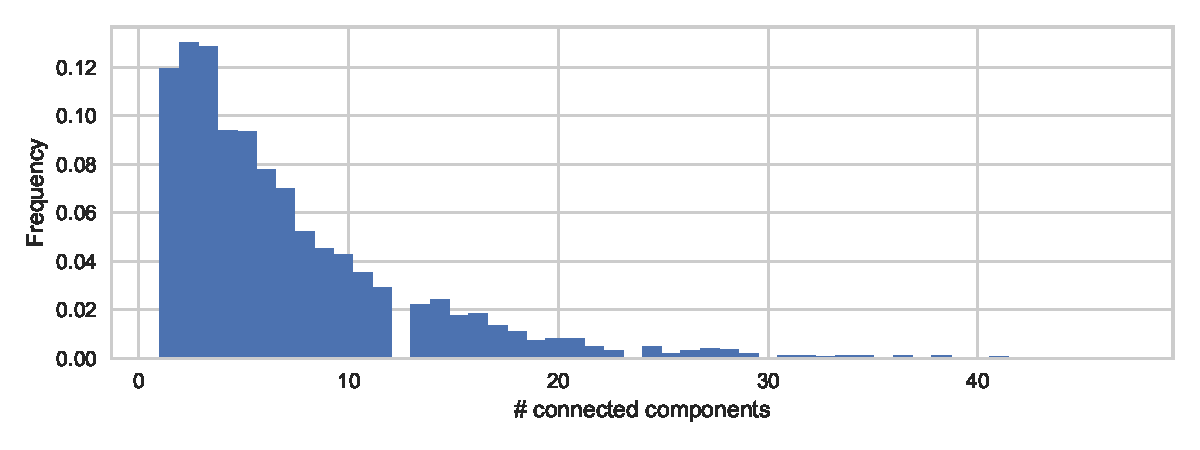
\includegraphics[width=0.8\linewidth]{assets/figures/hist-connected-components-ling-spam-CMap.pdf}
\caption[Statistics: Histogram of connected components per concept map]{Histogram of connected components per concept map. Dataset: \textit{ling-spam}.}\label{fig:histogram_connected_components}
\end{figure}

\begin{figure}[htb!]
    \centering
    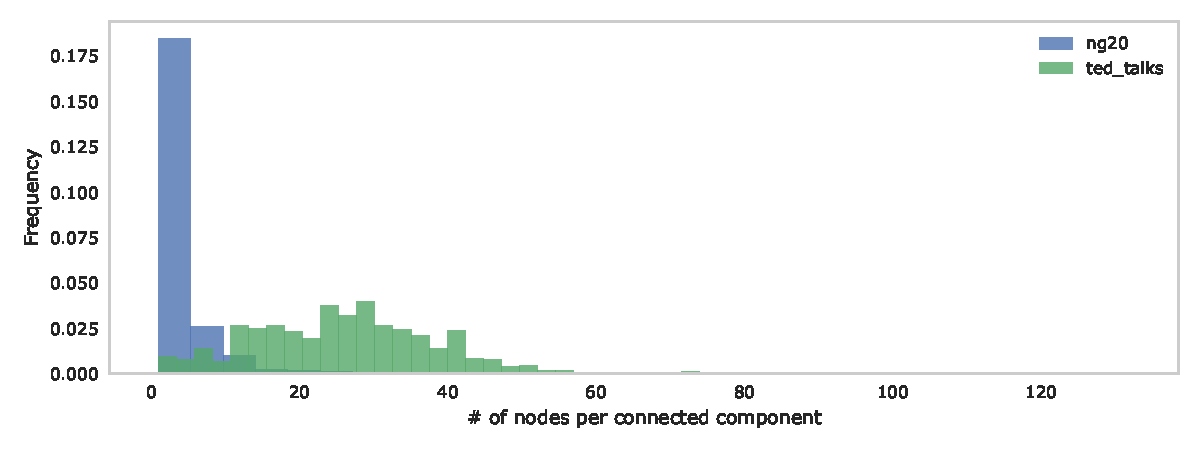
\includegraphics[width=0.9\linewidth]{assets/figures/connected_component_size_comparison.pdf}
    \caption[Statistics: Histogram of size of connectec components]{Histogram of the size of connected components, ie. the number of nodes per connected component, of concept maps for two datasets. The distribution of the size of connected components varies greatly between different datasets. In this instance, the \textit{ng20} dataset has mostly small connected components while the \textit{ted\_talks} dataset has bigger connected components. This is most likely due to the fact that the \textit{ted\_talks} dataset consists of longer, more coherent texts while the \textit{ng20} texts are shorter as well as more informal, leading to fewer recurring concepts.}
    \label{fig:histogram_connected_component_size}
\end{figure}

\begin{figure}[htb!]
\centering
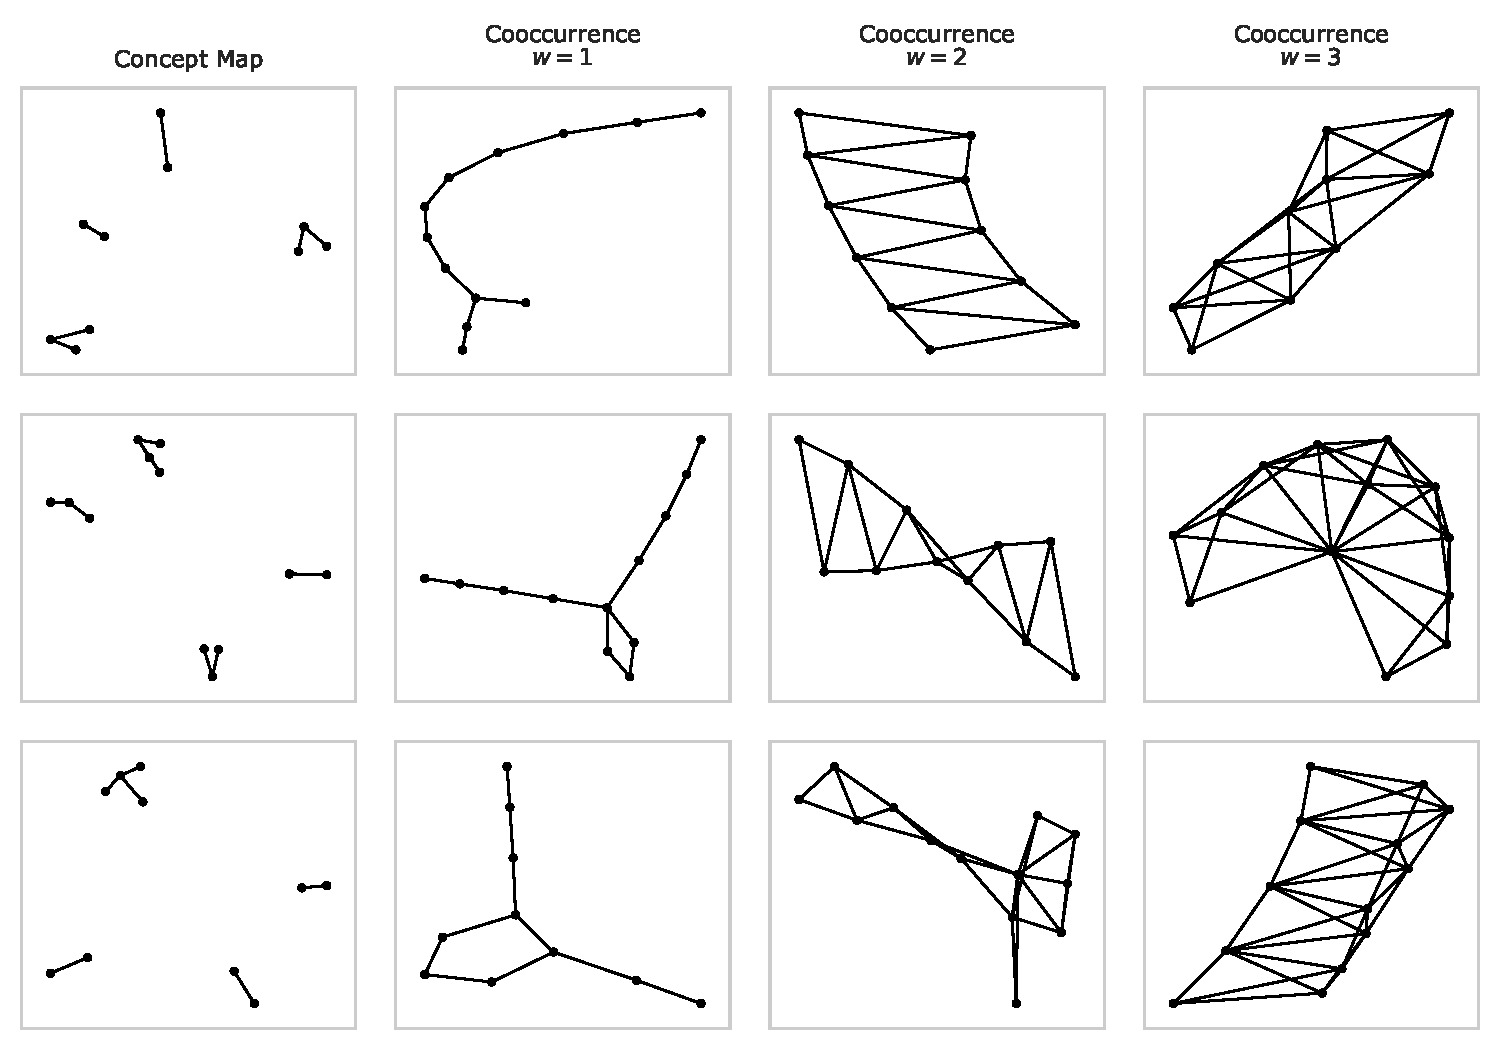
\includegraphics[width=0.8\linewidth]{assets/figures/examples_graphs.pdf}
\caption[Examples: Graph types]{Graph examples per type. Three random examples are shown per type. $w$ stands for the window size of the co-occurrence graph. The concept map examples all have more than one connected component, while all co-occurrence graphs have only one. The shown graphs were randomly chosen from all graphs with $5 \leq |V| \leq 10$.Dataset: \textit{ng20}}\label{fig:graph_examples}
\end{figure}

\begin{figure}[htb!]
\centering
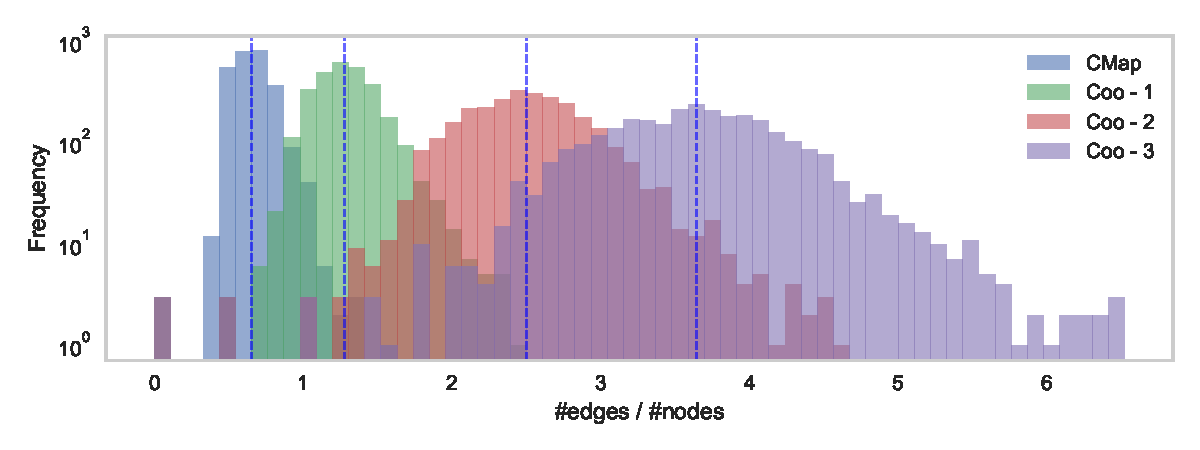
\includegraphics[width=0.7\linewidth]{assets/figures/hist-edgesnodes.pdf}
\caption[Statistics: Histogram of the number of edges divided by the number of nodes]{Histogram of the number of edges divided by the number of nodes. Per graph type. The lines correspond to the median value.}
\label{fig:histogram-edges-div-nodes-per-type}
\end{figure}

The co-occurrence graphs also have a simple structure.
Co-occurrence graphs are always connected, ie. the number of connected components is 1, or 0 in the case of an empty graph.
When the window size is 1, the graph is similar to a path, meaning that most of the nodes have a degree $< 2$. With increasing window size, the graph also gets more connected.

\answersummary{
Concept maps have a relatively homogeneous structure.
The bulk of its nodes have only a small number of neighbors.
The degrees of nodes are quite low, also hinting that there are few recurring concepts.
}